\documentclass[../main.tex]{subfiles}
\graphicspath{{\subfix{../../images/}}}

\begin{document}

To make sure that data sent from a device is received on the other side correctly, without errors, error correction must be done to make sure the data is valid. Here are some methods:

\begin{itemize}
    \item \textbf{Parity Checks:} This adds an extra bit (0 or 1) to a piece of data (usually a byte) based on the number of 1s already present. The number of 1s are totalled. Depending on if even or odd parity are agreed upon from the sender and receiver, if the number of 1s is even, the parity bit is 1, for odd parity the parity bit is 1 if the number of 1s is odd. If the receiver's calculated digit is the same as the digit sent, it indicates no error. However, this method can only detect single-bit errors and not multiple-bit errors.
    \item \textbf{Cyclic Redundancy Checks (Checksums, CRCs):} The data bits are added together, processed in a certain predetermined way, and the result (checksum) is appended to the data packet. The receiving device recalculates the checksum on the received data and compares it to the received checksum. If they match, the data is assumed to be error-free. This method is more robust than parity checks.
    \item \textbf{Echo Checks:} The sender sends the data packet and then waits for an exact copy of the packet back from the receiving device. This confirms successful data transfer but introduces a delay due to the back-and-forth communication.
\end{itemize}

\subsection{Parity Blocks}

These are like 2D parity checks. Each byte of data sent will have one bit used for parity, when the digit is calculated horizontally. Then, a whole other byte of data is also sent; with just parity bytes from parity checks from each vertical column.

\begin{figure}[h]
    \centering
    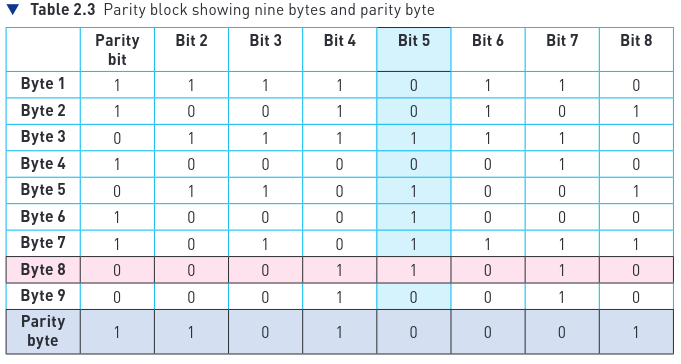
\includegraphics[width=0.7\textwidth]{parity_block.png}
    \caption{From the textbook. "[The table] shows how the data arrived at the receiving end. It is now necessary to check the parity of each byte horizontally (bytes 1 to 9) and vertically (columns 1 to 8). Each row and column where the parity has changed from even to odd should be flagged:"}
    \label{fig:parity_block}
\end{figure}

Figure \ref{fig:parity_block} from the textbook shows this. An extra byte of information is used as parity bits for each column, and each row has one data bit dedicated to storing horizontal parity data. This allows exact errors to be pinpointed (bit flips).

\subsection{Check Digits}

\subsubsection{ISBN-13}

\end{document}
